\begin{usecase}{Connect WhatsApp}
  \ucbasicinfo{Medium}{Regular}
  \ucshortdescription{This UC allows the user to connect their WhatsApp account to the system.}
  \uctrigger{This UC is triggered when the user clicks on ``Connect WhatsApp'' button in the app.}
  \ucactors{User}{WhatsApp}
  \ucpreconditions{User must be logged in}
  \ucrelationships{N/A}{N/A}{N/A}
  \ucinputsoutputs{
    \begin{itemize}
      \item \textbf{WhatsApp phone number} (Source: User)
      \item \textbf{WhatsApp linking code} (Source: User)
    \end{itemize}
  }{
    \begin{itemize}
      \item \textbf{WhatsApp auth credentials} (Destination: System)
    \end{itemize}
  }
  \ucmainflow{
    \begin{enumerate}
      \item The user clicks ``Connect WhatsApp'' button.
            \ucinfo{The system asks for the user's WhatsApp phone number.}
      \item The user enters their WhatsApp phone number.
            \ucinfo{WhatsApp shows the linking code in their app.}
      \item The user enters the linking code in our app.
            \ucinfo{The app shows a success screen if connection was sucessful.}
    \end{enumerate}
  }
  \ucalternateflows{
    \begin{itemize}
      \item If the WhatsApp connection fails, the user must redo the steps and try again.
      \item If the user enters a wrong linking code, the connection of the WhatsApp account will fail unless they enter the correct code.
    \end{itemize}
  }
  \ucexceptions{
    \begin{itemize}
      \item \textbf{Wrong linking code:} If the user enters a wrong linking code too many times, the connection of the WhatsApp account will fail.
      \item \textbf{Network issue:} A network issue interrupting the communication between the app, the server, and WhatsApp.
    \end{itemize}
  }
  \ucconclusion{The UC ends when the user has a connected WhatsApp account in the system.}
  \ucpostconditions{The system has access to the user's WhatsApp account.}
\end{usecase}

\begin{figure}[!h]
  \centering
  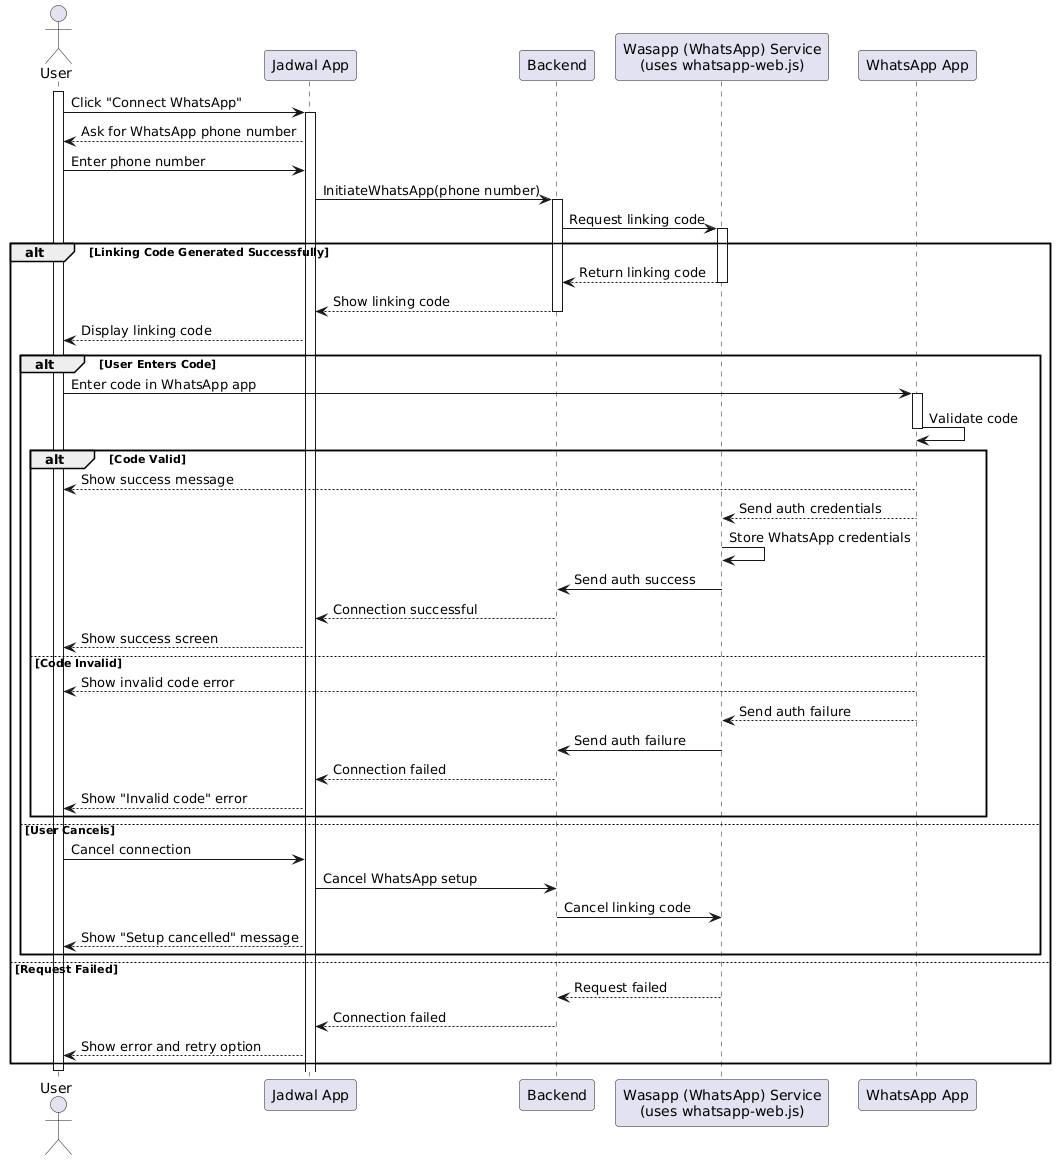
\includegraphics[width=\textwidth]{images/docs/diagrams/sequence-diagrams/all-sequence-diagrams/Connect WhatsApp.png}
  \caption{Connect WhatsApp Sequence Diagram}
  \label{fig:seq/connect-whatsapp}
\end{figure}

The "Connect WhatsApp Sequence Diagram", shown in \textbf{Figure~\ref{fig:seq/connect-whatsapp}}, illustrates the two-phase authentication process for connecting a user's WhatsApp account to Jadwal. The sequence begins with the InitiateWhatsApp gRPC call, where the user provides their phone number to the Backend.

The Backend then communicates with the WhatsApp service to request a linking code. This interaction follows two possible paths:

\begin{itemize}
  \item If the linking code request succeeds:
        \begin{enumerate}
          \item The user receives the linking code in their WhatsApp application
          \item The user initiates the CompleteWhatsApp gRPC call with the linking code
          \item The Backend validates the code with WhatsApp
          \item Upon successful validation, the WhatsApp authentication credentials are securely stored in the Database for future use
        \end{enumerate}
  \item If the linking code request fails:
        \begin{itemize}
          \item The Backend immediately returns an InitiateWhatsApp failure response to the user
        \end{itemize}
\end{itemize}

During the completion phase, if the linking code validation fails, the Backend returns a CompleteWhatsApp failure response, requiring the user to restart the process. This secure two-phase authentication ensures that only legitimate WhatsApp account owners can connect their accounts to Jadwal while maintaining the integrity of the WhatsApp integration.